\chapter{Evaluation}
\thispagestyle{fancy}
\label{chap:Evaluation}

\noindent
In diesem Kapitel werden die Experimente umfangreich evaluiert. Dies geschieht einerseits automatisiert auf Basis der ausgewählten Metriken, andererseits manuell in Form einer qualitativen Analyse der aus den Anhängen A und B generierten Zusammenfassungen. Die Experimente werden zwecks anschließender Zuordnung wie folgt kodiert:

\begin{table}[htb]
\centering
\begin{tabular}{ | p{1cm} | p{7.5cm} | }
\hline
\textbf{ID} & \textbf{Experiment} \\
\hline
1 & Reproduktion auf englischen Daten \\
\hline
2 & Adaption auf deutschen Daten \\
\hline
3 & Adaption auf multilingualen Daten \\
\hline
\end{tabular}
\caption{Kodierung der Experimente.}
\label{table:ExpCoding}
\end{table}


\section{Automatische Auswertung}
\noindent
In \autoref{table:ExpEvaluation} sind die \ac{ROUGE}-Scores der \ac{TF2TF} aller Experimente gesamtheitlich dokumentiert. Dabei ist die Konfiguration der Experimente jeweils anhand der ID, der genutzten \ac{DLR} und der Sprache der eingegangenen Textdaten nachvollziehbar. Die drei letztgenannten Spalten sind als zusammengesetzter Primärschlüssel zu verstehen.

\begin{table}[htb]
\centering
\begin{tabular}{ | p{1cm} | p{2.5cm} | p{2.5cm} | p{2.5cm} | p{2.5cm} | p{2.5cm} | }
\hline
\textbf{ID} & \textbf{DLR} & \textbf{Sprache} & \textbf{R-Recall} & \textbf{R-Precision} & \textbf{R-Measure} \\
\hline
1 & BERT & EN & 15.78 & 10.25 & 12.11 \\
\hline
1 & XLM-R & EN & 16.49 & 17.12 & 16.25 \\
\hline
2 & BERT & DE & 15.93 & 10.52 & 11.97 \\
\hline
2 & XLM-R & DE & 15.93 & 10.32 & 11.86 \\
\hline
3 & BERT & EN \& DE & 16.76 & 11.18 & 12.68 \\
\hline
3 & XLM-R & EN \& DE & 16.44 & 15.45 & 15.35 \\
\hline
3 & BART & EN \& DE & 15.01 & 12.43 & 13.10 \\
\hline
\end{tabular}
\caption{Ergebnisse im Experimentvergleich.}
\label{table:ExpEvaluation}
\end{table}

\noindent
\textbf{Experiment 1: Reproduktion auf englischen Daten}\\
\noindent
Im ersten Experiment geschah die Reproduktion des \ac{SOTA} auf Basis englischsprachiger Textdaten. Das \ac{TF2TF} ist demnach unter Nutzung von \ac{BERT} und \ac{XLM-R} weitestgehend \ac{SOTA}-konform. Im Bereich der \ac{XLM-R} ist jedoch ein ungewöhnlich hoher R-Precision-Score auffallend, welcher sich in der Berechnung auch auf den R-Measure-Score auswirkt. Dies bedeutet per Formel eine hohe Übereinstimmung zwischen den Wörtern der Originaltexte und der generierten Zusammenfassungen. Eine weitergehende Ursache hierfür wird im nachfolgenden Kapitel ergründet. Die Lernfortschritte sind anhand der Fehlerentwicklung in \autoref{pic:ExpEnLoss} visualisiert. Hierbei ist zu erkennen, dass \ac{XLM-R} erst spät, dann aber ebenbürtig lernt.\\

\begin{figure}[h]
  \centering
  \fbox{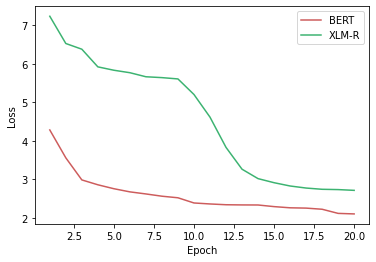
\includegraphics[width=0.55\linewidth]{./source/images/lossenglish.png}}
  \caption{Loss in der SOTA-Reproduktion im Modellvergleich.}
  \label{pic:ExpEnLoss}
\end{figure}

\noindent
\textbf{Experiment 2: Adaption auf deutschen Daten}\\
\noindent
Im zweiten Experiment geschah erstmalig die sprachtechnische Adaption der \ac{TF2TF}. Hierfür kamen demnach ausschließlich deutschsprachige Daten zum Einsatz. \autoref{table:ExpEvaluation} gibt hierbei zu erkennen, dass das Modell unter Nutzung von \ac{BERT} qualitativ in Englisch genauso gut wie in Deutsch ist. Im Bereich der \ac{XLM-R} sind nun keine auffallenden Werte mehr zu verzeichnen. Wertmäßig gleichen sich die \ac{TF2TF} nun unter Nutzung beider \ac{DLR} unter Akzeptanz eines gewissen Rauschens auf \ac{SOTA}-Niveau. Die Lernfortschritte sind in bekannter Weise in \autoref{pic:ExpDeLoss} visualisiert.
\newpage

\begin{figure}[h]
  \centering
  \fbox{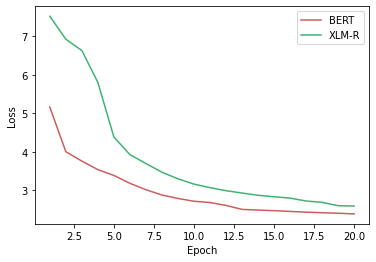
\includegraphics[width=0.55\linewidth]{./source/images/lossgerman.png}}
  \caption{Loss in der Adaption auf deutschen Daten im Modellvergleich.}
  \label{pic:ExpDeLoss}
\end{figure}

\noindent
\textbf{Experiment 3: Adaption auf multilingualen Daten}\\
\noindent
Im dritten Experiment geschah die sprachtechnische Adaption der \ac{TF2TF} auf Basis multilingualer Textdaten. \ac{BART} wird indes aus externer Quelle bezogen. Die Evaluation geschieht im Kontext dieser Arbeit ausschließlich auf deutschsprachigen Textdaten. In \autoref{table:ExpEvaluation} wird ersichtlich, dass sich das Modell unter Nutzung von \ac{BERT} nun über den \ac{SOTA} hinaus verbessert, während im Bereich der \ac{XLM-R} erneut auffallende Werte entstehen. \ac{BART} entspricht ebenfalls dem \ac{SOTA}. Hier sei jedoch angemerkt, dass er den \ac{SOTA} auf Basis einer englischsprachigen Evaluation übersteigt. In \autoref{pic:ExpMlLoss} ist abermals die recht späte Konvergenz der \ac{XLM-R} nachvollziehbar, welche womöglich auf die architektonischen Unterschiede der \ac{DLR} zurückzuführen ist.\\

\begin{figure}[h]
  \centering
  \fbox{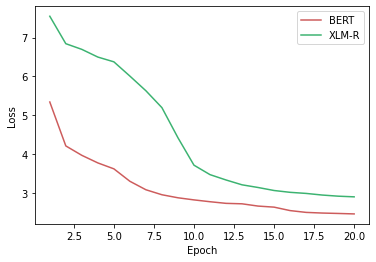
\includegraphics[width=0.55\linewidth]{./source/images/lossmultilingual.png}}
  \caption{Loss in der Adaption auf multilingualen Daten im Modellvergleich.}
  \label{pic:ExpMlLoss}
\end{figure}
\newpage


\section{Qualitative Analyse}
\noindent
Die soeben wertmäßig evaluierten Experimente werden nun ergänzend qualitativ analysiert. Hierfür werden die \ac{TF2TF} aller Experimente sprachabhängig entweder Anhang A oder Anhang B unterzogen, indem die dort enthaltenen mitunter herausfordernden Texte maschinell zusammengefasst und subjektiv bewertet werden. Eine derartige Analyse ist erforderlich, um die Qualität sowie die praktische Eignung der trainierten \ac{TF2TF} vollends beurteilen zu können. Die qualitative Analyse ist außerdem erforderlich, um den teilweise kritisch begutachteten sowie statistisch veranlagten \ac{ROUGE}-Score qualitativ einzuordnen. Zudem sei bemerkt, dass die in diesem Kapitel referenzierten Zusammenfassungen in englischer und deutscher Sprache modellübergreifend stets den Anhängen C und D zu entnehmen sind.\\

\noindent
\textbf{Experiment 1: Reproduktion auf englischen Daten}\\
\noindent
Ergänzend zum ersten Experiment ist nun zu analysieren, ob das \ac{TF2TF} unter Nutzung von \ac{BERT} tatsächlich \ac{SOTA}-konform ist und wie die auffallenden Werte unter Nutzung von \ac{XLM-R} zu erklären sind.\\

\noindent
\ac{BERT} scheint die beispielhaften Texte sehr gut verstehen zu können. Dies war zu erwarten, da \ac{BERT} bekanntermaßen hervorragend als Encoder funktioniert, etwas beschwerlicher hingegen als Decoder. Dies ist jedoch bis auf eine Ausnahme im Text über das Finale der WM 2014 nicht herauszulesen. Dabei sind die entsprechenden Zusammenfassungen nicht zur orthographisch und grammatikalisch korrekt, sondern weitestgehend auch mit den wichtigsten Informationen ausgestattet. Das \ac{TF2TF} unter Nutzung von \ac{BERT} gilt daher tatsächlich als \ac{SOTA}-konform.\\

\noindent
\ac{XLM-R} verspricht eine wertmäßige Verbesserung. In den generierten Zusammenfassungen wird die inhaltliche Unzulänglichkeit jedoch für den menschlichen Leser auch ohne Kenntnis über die ursprünglichen Texte sehr schnell deutlich. Gleichermaßen ist hier nachvollziehbar, wie die hohen Werte im Bereich der R-Precision und der R-Measure entstanden sind: Die als wichtig erkannten Worte oder Wortpassagen der ursprünglichen Texte werden in den Zusammenfassungen sehr häufig wiederholt. Diese Form der Exploitation hat im Kontext der \ac{ATS} einen höchst nachteiligen Effekt, da inhaltlich keine qualitativen Zusammenfassungen entstehen. Die gegenüber \ac{BERT} komplexere Architektur der \ac{XLM-R} scheint mit den zugeführten Textdaten nicht korrekt lernen zu können und gilt hiermit nicht mehr als \ac{SOTA}-konform.
\newpage

\noindent
\textbf{Experiment 2: Adaption auf deutschen Daten}\\
\noindent
Ergänzend zum zweiten Experiment ist zu analysieren, ob die Adaption der \ac{TF2TF} unter Nutzung von \ac{BERT} und \ac{XLM-R} auf deutschen Daten qualitativ ist. \ac{BERT} scheint die beispielhaften Texte trotz gleichbleibender Werte mit vermehrt fehlerhaften sowie teils widersprüchlichen Informationen zusammenzufassen. Dies ist auch gleichbleibend, wenn \ac{BERT} durch \ac{GBERT} ausgetauscht wird. \ac{XLM-R} weist trotz normalisierter Werte auf \ac{SOTA}-Niveau ein ähnlich fehlerbehaftetes Verhalten auf.\\

\noindent
Hierbei wird einerseits die Abhängigkeit der Modelle vom Umfang der Textdaten deutlich. Dies betrifft sowohl das Vortraining der verwendeten \ac{DLR} als auch das Fine-Tuning der \ac{TF2TF}. Dabei stehen in englischer Sprache so viele Textdaten wie in keiner anderen Sprache frei zur Verfügung. Folglich ist es nicht verwunderlich, wenn die verborgenen Strukturen anderer Sprachen nicht vollends erlernt werden können und die Qualität dadurch limitiert wird.\\

\noindent
Andererseits wird die Abhängigkeit der Modelle von der Beschaffenheit der Textdaten deutlich, insbesondere anhand der Natur der Zusammenfassungen. Hier ist nämlich ein typisches Element der Nachrichtendomäne erkennbar, da anstatt einer konventionellen Zusammenfassung oftmals ein Teaser generiert wird, der den Leser binden und zum eigentlichen Text weiterleiten soll. Dieses Verhalten ist jedoch nicht auf das Modell zurückzuführen, sondern auf die Trainingsdaten, welche größtenteils eben jener Nachrichtendomäne entstammen. Dies unterstreicht insgesamt die Notwendigkeit einer intensiven Datenanalyse. Hinsichtlich eines praktischen Einsatzes ist also stets ein anforderungsgerechter Korpus zu formieren. Zudem ist der Einfluss des vortrainierten Modells bemerkbar, beispielsweise im Text über das Finale der WM 2014. Hier wird im originalen Text von Jogi Löw geschrieben, in der Zusammenfassung hingegen von Jürgen Klopp. Letzterer wurde zuvor jedoch nie erwähnt. Dies kann mit der geringen Distanz beider Personen im Vektorraum erklärt werden und ist somit zwar sachlogisch falsch, mathematisch jedoch nachvollziehbar. Dies tritt in ähnlicher Weise auch in den anderen Zusammenfassungen auf. Ein Fine-Tuning mit sehr viel mehr Trainingsdaten verspricht dieses Rauschen hinreichend zu minimieren.
\newpage

\noindent
\textbf{Experiment 3: Adaption auf multilingualen Daten}\\
\noindent
Ergänzend zum dritten Experiment ist zu analysieren, inwiefern wie wertmäßigen Fortschritte auch in den generierten Zusammenfassungen erkennbar sind. Außerdem ist erstmalig die Qualität von \ac{BART} zu untersuchen.\\

\noindent
Das \ac{TF2TF} unter Nutzung von \ac{BERT} verbessert sich in Englisch nun bis hin zur praktischen Eignung, in Deutsch jedoch nicht. Das \ac{TF2TF} unter Nutzung von \ac{XLM-R} erzielt hingegen keine Verbesserung. Dies ist vermutlich auf die erneut ungewöhnlich hohen Werte im Bereich der R-Precision und der R-Measure zurückzuführen. \ac{XLM-R} scheint große Probleme mit den vorliegenden englischsprachigen Textdaten zu haben.\\

\noindent
\ac{BART} weist aufgrund der identischen Datengrundlage ein ähnliches Verhalten wie die monolingualen \ac{TF2TF} auf, scheint jedoch insgesamt robuster zu sein und weniger Fehler zu machen. Dennoch sind auch hier inhaltliche Mängel sowie erstmalig auch englische Wörter in deutschen Zusammenfassungen zu verzeichnen. Entgegen obig formulierter Erwartung scheint \ac{BART} dem lockenden Element der Nachrichtendomäne nicht nachzukommen. \ac{BART} ist für die \ac{ATS} in englischer Sprache das beste Modell, in deutscher Sprache vermutlich nur mit einem hinreichenden Fine-Tuning. \ac{BERT} ist wertmäßig und subjektiv wider Erwarten nur leicht unterlegen.\\

\noindent
Die Ergebnisse wurden nun nicht nur evaluiert und analysiert, sondern teilweise bereits bewertet und begründet. Dies wird nachfolgend hinreichend fortgeführt.
